\documentclass{standalone}
\usepackage[all]{xy}
\usepackage{bm}
\usepackage{tikz}

\usetikzlibrary{shapes.arrows, shapes.geometric}
\tikzstyle{line} = [thick,->]
\tikzstyle{arrow} = [
	thick,
	->,
	>=stealth,
	black,
]
\tikzstyle{agente} = [
	rectangle, 
	minimum width=1cm, 
	minimum height=1cm,
	text centered,
	draw=black, 
	fill=green!30
]
\tikzstyle{modelo} = [
	rectangle, 
	rounded corners,
	minimum width=1cm, 
	minimum height=1cm,
	text centered,
	draw=black, 
	fill=red!30
]
\tikzstyle{memoria} = [
	rectangle, 
	rounded corners,
	minimum width=1cm, 
	minimum height=1cm,
	text centered,
	draw=black, 
	fill=gray!30
]
\tikzstyle{entorno} = [
	rectangle, 
	minimum width=1cm, 
	minimum height=1cm,
	text centered, 
	draw=black, 
	fill=blue!15
]


\begin{document}

\begin{tikzpicture}
\node(A) at (0,4) {\txt{History\\
\includegraphics[width=1cm]{history_2.png}\\len=1}};
\node(B) at (-4,0) {\txt{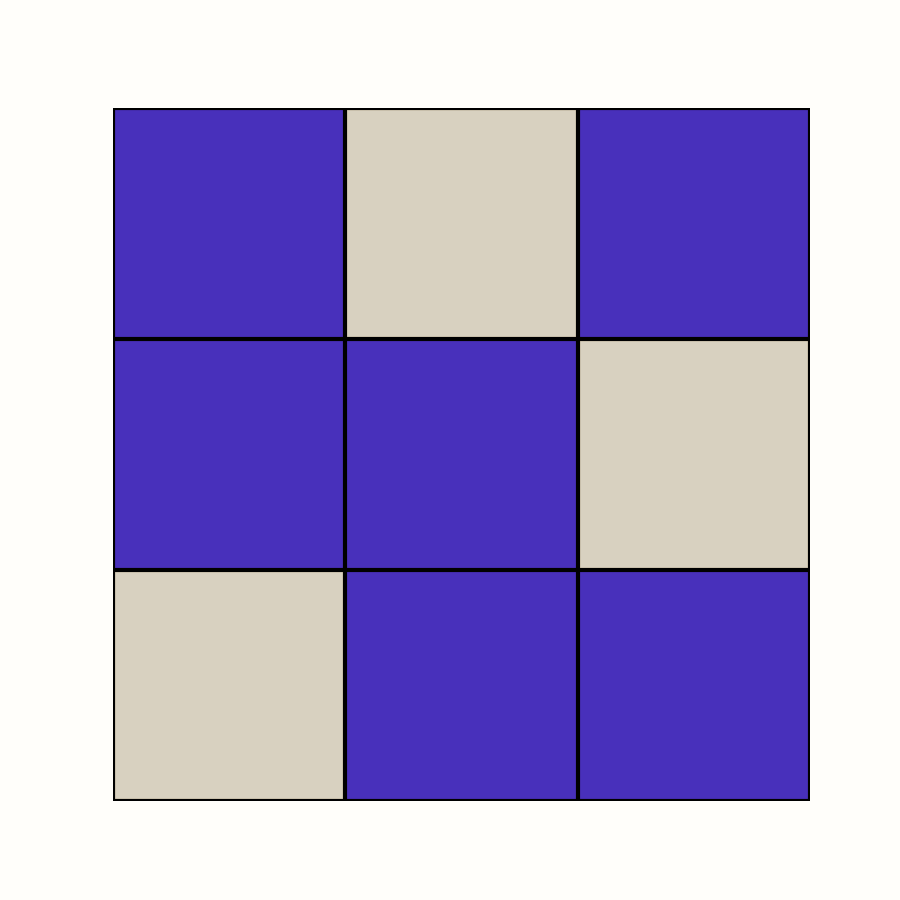
\includegraphics[width=3cm]{FRA_region_1.png}\\Focal region}};
\node(C1) at (-4.8, 1.65) {};
\node(C2) at (-3.9, 1.55) {};
\node(C3) at (-3.1, 1.45) {};

\node(M) at (2, 4.75) {player 1};
\node(Mh1) at (0.5, 4.75) {};
\node(Mh2) at (6, 4.75) {};
\draw [->] (M) -- (Mh1);
\draw [->] (M) -- (Mh2);


\draw [black!30, thick, dashed] (-5.2, 1.65) rectangle (-4.3,-1);
\draw [black, thick, dashed] (-4.4, 1.55) rectangle (-3.5,-1.1);
\draw [black!30, thick, dashed] (-3.7, 1.45) rectangle (-2.7,-1.2);

\draw[arrow, black!30, line width=1.5pt] (A) edge [out=180, in=90, anchor=south east] node {$0.33$} (C1);
\draw[arrow, black, line width=1.5pt] (A) edge [out=180, in=90, anchor=east] node {$1${\color{black}.}} (C2);
\draw[arrow, black!30, line width=1.5pt] (A) edge [out=180, in=90, anchor=west] node {$0.33$} (C3);

\node(AA) at (7,4) {\txt{History\\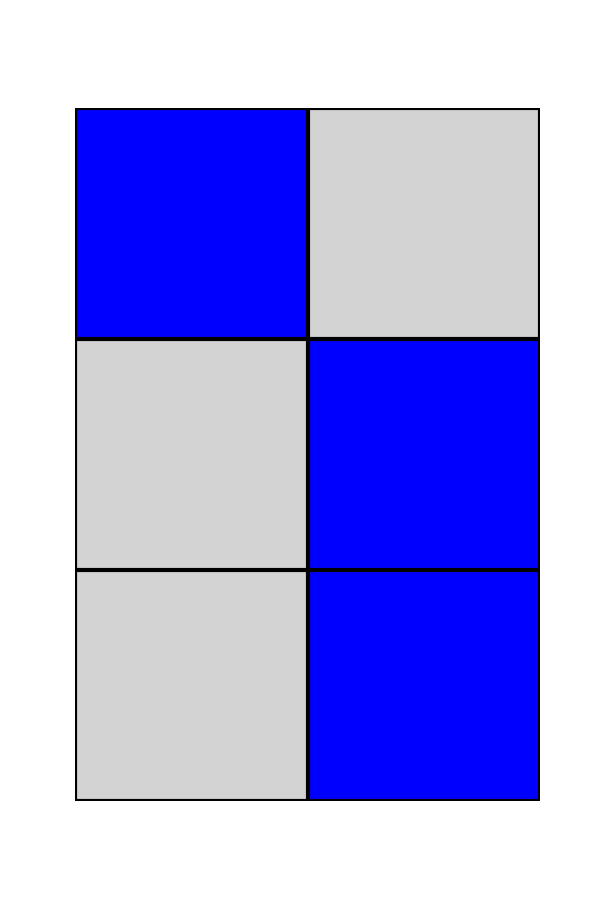
\includegraphics[width=2cm]{history_1.png}\\len=2}};
\node(AB) at (3,0) {\txt{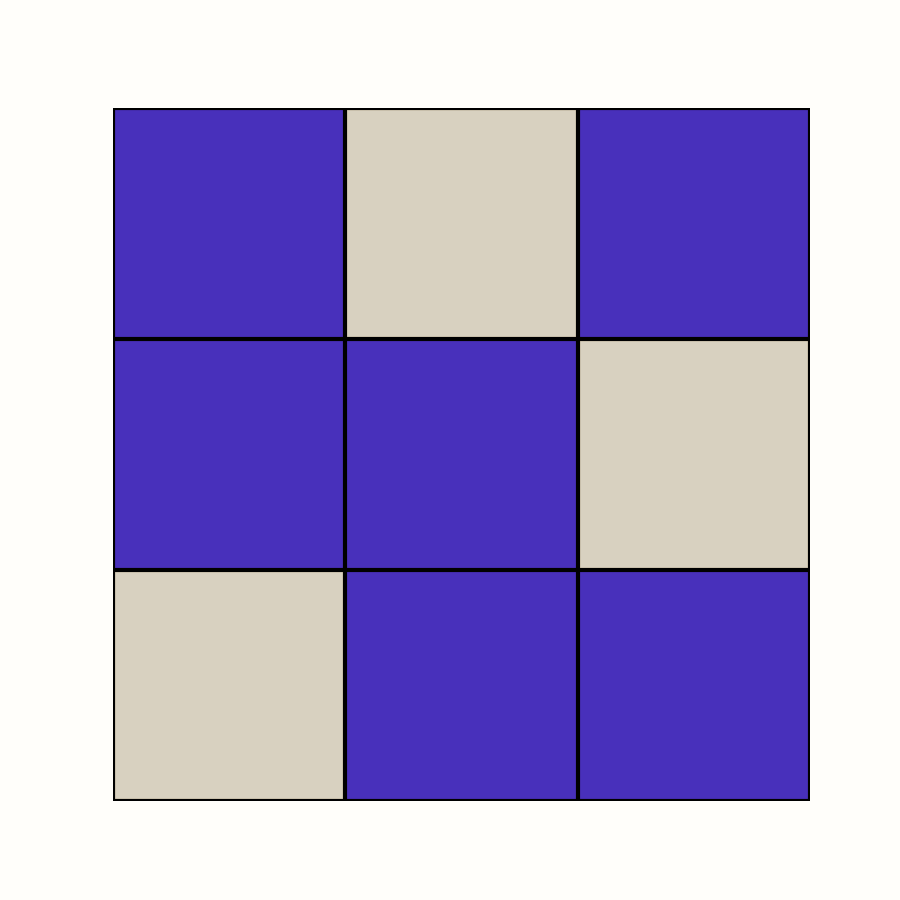
\includegraphics[width=3cm]{FRA_region_1.png}\\Focal region}};
\node(AB1) at (4.6,0.2) {
\includegraphics[width=0.77cm]{FRA_region_2.png}\\};
\node(AC1) at (2.5, 1.65) {};
\node(AC2) at (3.7, 1.55) {};
\node(AC3) at (4.6, 1.45) {};

\draw [black!83, thick, dashed] (1.8, 1.65) rectangle (3.5,-1);
\draw [black!17, thick, dashed] (2.6, 1.55) rectangle (4.3,-1.1);
\draw [black!50, thick, dashed] (3.2, 1.45) rectangle (5.1,-1.2);

\draw[arrow, black!83, line width=1.5pt] (AA) edge [out=180, in=90, anchor=south east] node {$0.83$} (AC1);
\draw[arrow, black!17, line width=1.5pt] (AA) edge [out=180, in=90, anchor=east] node {$0.17$} (AC2);
\draw[arrow, black!50, line width=1.5pt] (AA) edge [out=180, in=90, anchor=west] node {$0.5$} (AC3);

\node(D1) at (-3.2, 1) {};
\node(D2) at (-0.6, -2.5) {\{don't go=0, go=1\}};
\draw[black, line width=1.5pt, ->] (D1) edge [out=0, in=90] (D2);

\node(AD1) at (3.8, 1) {};
\node(AD2) at (5, -2.5) {\{don't go=0.17, go=0.83\}};
\draw[black, line width=1.5pt, ->] (AD1) edge [out=0, in=90] (AD2);

\node(S) at (2, -5) {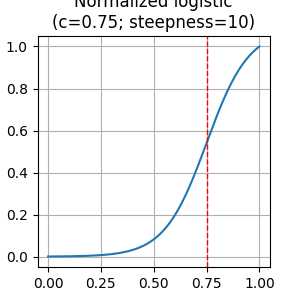
\includegraphics[width=3cm]{logistic.png}};

\node(BD2) at (-0.6, -7.5) {\{don't go=0, go=1\}};
\draw[black, line width=1.5pt, ->] (D2) edge [out=270, in=90] (BD2);

\node(CD2) at (5, -7.5) {\{don't go=0.00, go=0.2\}};
\draw[black, line width=1.5pt, ->] (AD2) edge [out=270, in=90] (CD2);

\node(1) at (-1.5, 5.5) {\textbf{A}};
\node(2) at (-4.75, 3.75) {\textbf{B}};
\node(3) at (-0.5, 0) {\textbf{C}};
\node(4) at (-1.5, -5) {\textbf{D}};


\end{tikzpicture}

\end{document}